\section{Motivation}
\label{sec:motivation}

In this section, we motivate our ideas via an example written in
\txnimp - a functional language equipped with a \C{DB} monad to
compose database computations. Besides the usual \C{bind} and
\C{return} combinators, monad offers an \C{atomically} combinator that
executes a database computation and returns the result. 

\begin{figure}
\centering
\begin{ocaml}
let new_order_ d_id c_id item_reqs = atomically do
  dist <- SQL.select1 District (fun d -> d.d_id = d_id);
  let o_id = dist.d_next_o_id;
  SQL.update District (fun d -> {d with d_next_o_id =d_next_o_id + 1})
                      (fun d -> d.d_id = d_id );
  SQL.insert Order {o_id=o_id;  o_d_id=d_id; 
                    o_c_id=c_id; o_ol_cnt=S.size item_reqs; };
  foreach item_reqs @@ fun item_req -> do
    stk <- SQL.select1 Stock (fun s -> s.s_i_id = item_req.ol_i_id);
    let s_qty' = if stk.s_qty >= item_req.ol_qty + 10 
                then stk.s_qty - item_req.ol_qty 
                else stk.s_qty - item_req.ol_qty + 91;
    SQL.update Stock (fun s -> {s with s_qty = s_qty'}) 
                     (fun s -> s.s_i_id = item_req.ol_i_id);
    SQL.insert Order_line {ol_o_id=o_id; ol_d_id=d_id; 
                           ol_i_id=item_req.ol_i_id; ol_qty=item_req.ol_qty}
 
\end{ocaml}
\caption{\small Concurrent withdraw transactions}
\label{fig:new_order_code}
\vspace*{-10pt}
\end{figure}

Fig.~\ref{fig:new_order_code} shows a simplified version of the TPC-C
\C{new\_order} transaction written in \txnimp (the \C{do} syntax ala
Haskell is used for convenience). TPC-C is an Online Transaction
Processing (OLTP) benchmark that models an order-processing system for
a wholesale parts supply business. The business logic is captured in 5
database transactions that operate on 9 tables. \C{new\_order} is one
such trasaction that operates on \C{District}, \C{Order},
{New\_order}, \C{Stock}, and \C{Order\_line} tables. The transaction
acts on the behalf of a customer, whose id is \C{c\_id}, to place a
new order for the given set of items (\C{item\_reqs}), to be served by
a warehouse under the district identified by \C{d\_id}. The
transaction does so by invoking appropriate SQL functionality,
captured in Fig.~\ref{fig:new_order_code} by various calls to
functions under the \C{SQL} module. All \C{SQL} functions take the
table name (a nullary constructor) as their first argument. The
higher-order \C{SQL.select1} function accepts a boolean function that
describes the selection criteria, and returns any record that meets
the criteria (it models the SQL query \C{SELECT \ldots\xspace LIMIT
1}). \C{SQL.update} also accepts a boolean function (3rd argument) to
select the records to be updated. Its 2nd argument is a function that
maps each selected record to a new (updated) record. \C{SQL.insert}
inserts a given record into the specified table in the database.

The \C{new\_order} transaction inserts a new \C{Order} record, whose
id is the sequence number of the next order under the given district
(\C{d\_id}). The sequence number is stored in the corresponding
\C{District} record, and updated each time a new order added to the
system. Since each order may request multiple items (\C{item\_reqs}),
an \C{Order\_line} record is created for each requested item to relate
the order with the item. Each item has a corresponding record in the
\C{Stock} table, which keeps track of the quantity of the item left in
stock (\C{s\_qty}). The quantity is updated by the transaction to
reflect the processing of new order (if the stock quantity falls below
10, it is automatically replenished by 91).

TPC-C defines multiple invariants, called \emph{consistency
conditions}, over the state of the application in the database. One
such consistency condition is the requirement that for a given order
\C{o}, the order-line-count field (\C{o.o\_ol\_cnt}) should reflect
the number of order lines under the order, i.e., the number of
\C{Order\_line} records whose \C{ol\_o\_id} is equal to \C{o.o\_id}.
In a sequential exectution, it is more-or-less easy to see how this
condition condition is preserved by the \C{new\_order} transaction by
examining Fig.~\ref{fig:new_order_code}. A new \C{Order} record is
added with its \C{o\_id} distinct from the existing order ids, and its
\C{o\_ol\_cnt} set equal to the size of \C{item\_reqs} set. The
\C{foreach} loop runs once for each \C{item\_req}, adding a new
\C{Order\_line} record for each requested item, with its \C{ol\_o\_id}
field set to \C{o\_id}. Thus, by the end of the loop, the number of
\C{Order\_line} records in the database, whose \C{ol\_o\_id} is equal
to \C{o\_id}, is equal to the size of the \C{item\_req} set, which
inturn is equal to the \C{Order} record's \C{o\_ol\_cnt} field. Thus
the consistency condition is preserved. 

While the aforementioned reasoning is simple to perform manually, the
sequential verification of database programs, such as the one in
Fig.~\ref{fig:new_order_code}, is difficult to automate owing to the
presence of loops and collections. Thus verification of serializable
transactions is comparable to the verification of sequential
(imperative) programs in terms of difficulty. It is therefore not
unreasonable to expect the reasoning machinery (i.e., program logics
and inference techniques) developed for imperative programs to be
equally effective on serializable transactions.

Unfortunately, transactions are rarely serializable in practice, and
presence of weak isolation significantly complicates the reasoning
about database programs. Weak isolation allows a transaction to
witness the effects of concurrent transactions during its
execution\footnote{Weak isolation doesn't violate atomicity as long as
the witnessed effects are those of the committed transactions}.
Various levels of weak isolation differ in what effects each allows
the transaction to witness, and when. Admitting interference from
concurrent transactions may violate the invariants that would
otherwise hold under a fully isolated execution. 

Let us reconsider the \C{new\_order} transaction, which has been
previously shown to preserve TPC-C's consistency condition under a
serializable execution. However, serializability is rarely the default
isolation level on databases. For instance, the default on Postgres is
Read Committed (RC), which is considerably weaker than
serializability. An RC transaction is isolated from \emph{dirty
writes}, i.e., writes of uncommitted transactions, but is allowed to
witness the writes of concurrent transactions as soon as they are
committed. Thus, with two concurrent instances of the \C{new\_order}
transaction (call them $T_1$ and $T_2$) trying to place new orders for
different customers under the same district (\C{d\_id}), executions
shown in Fig.~\ref{fig:new_order_execs} are possible on Postgres.

\begin{figure}[!h]
\centering
\subcaptionbox {
  {\sc rc} Execution 1
  \label{fig:motiv-eg-1-a}
} [
  0.55\columnwidth
] {
  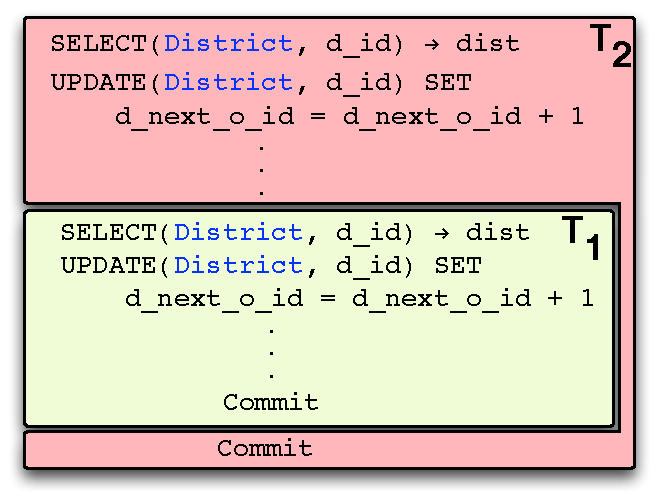
\includegraphics[scale=0.6]{Figures/motiv-eg-1-a}
}
%\hspace*{0.5in}
\subcaptionbox {
  {\sc rc} Execution 2
  \label{fig:motiv-eg-1-b}
}{
  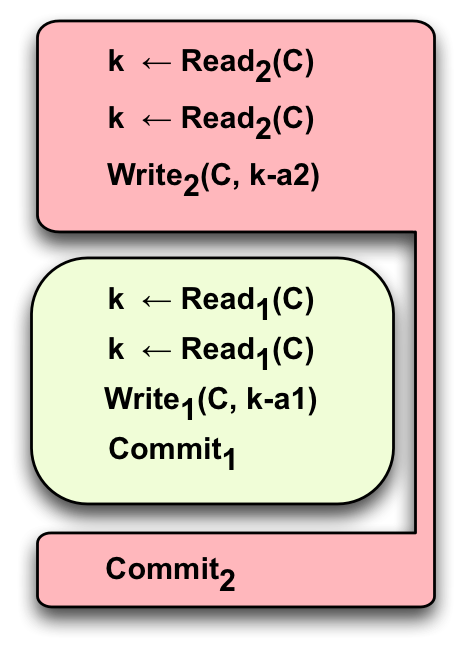
\includegraphics[scale=0.6]{Figures/motiv-eg-1-b}
}
\caption{\small A possible execution of the program shown in Fig.~\ref{fig:motiv-eg-1} under
  \iso{Read Committed} isolation level. Transaction \C{Wd1} is shown
  against lighter green background, and transaction \C{Wd2} against
  darker red background. Each transaction reads the balance (\C{B})
  twice, hence two \C{Reads}.}
\label{fig:rc-ex}
\end{figure}

The figure depicts an execution as a series of read, write, and commit
operations. In the execution on left, the \C{new\_order} instance
$T_1$ (green) reads the \C{d\_next\_o\_id} field of the district
record for \C{d\_id}, but before it increments the field, another
\C{new\_order} instance ($T_2$) begins its execution and commits. Note
that $T_2$ reads the same \C{d\_next\_o\_id} value as $T_1$, and
inserts new \C{Order} and \C{Order\_line} records with their \C{o\_id}
and \C{ol\_o\_id} fields (resp.) equal to \C{d\_next\_o\_id}. $T_2$
also increments the \C{d\_next\_o\_id} field, which $T_1$ has already
acccessed. This is allowed because reads do not obtain a mutually
exclusive lock on most databases, including Postgres. Post $T_2$'s
commit, $T_1$ resumes execution and adds new \C{Order} and
\C{Order\_line} fields with the same order id as $T_1$. Thus, by the
end of the execution, \C{Order\_line} records inserted by $T_1$ and
$T_2$ all bear the same order id. There are also two \C{Order} records
with the same district id (\C{d\_id}) and order id, none of whose
\C{o\_ol\_cnt} reflects the actual number of \C{Order\_line} records
inserted with that order id. This clearly violates TPC-C's consistency
condition.

Note that, in the above example, there is no Write-Write conflict, or
the \emph{lost update} anomaly that often characterizes concurrency
bugs, such as illegal concurrent withdraws on a bank
account~\cite{poloniexbug}. While $T_1$ and $T_2$ both increment the
\C{d\_next\_o\_id} field of the district record, they do so atomically
(Line 4 of Fig.~\ref{fig:new_order_code}), allowing both updates to be
present in the final state. Likewise, four other well-known anomalies
that characterize RC isolation~\cite{berenson}, namely, \emph{fuzzy
reads}, \emph{phantom reads}, \emph{read skew}, and \emph{write skew},
are also not exhibited by the example. Thus, any program analysis,
static or dynamic, that aims to determine appropriate isolation by
checking for possible manifestations of known anomalies fails to
identify grounds for promoting the isolation level of \C{new\_order}.
Yet, if we take the semantics of the application into account, it is
clear that RC is not an appropriate isolation level for
\C{new\_order}. Clearly, there is a need for a high-level verification
framework that lets us reason about transaction semantics in
conjunction with the semantics of weak isolation.

Facilitating high-level reasoning about weak isolation is however not
easy owing to the low-level nature of its specification, either in
terms of the implementation details~\cite{gray}, allowed
anomalies~\cite{berenson}, or well-formedness condition on program
traces~\cite{adyaphd,gotsmanconcur15}. For instance, does promoting
the isolation level of \C{new\_order} to Repeatable Read (RR) help in
preserving the consistency condition? To answer this question, one has
to relate the low-level specification of RR given in terms of
trace-based relations~\cite{adyaphd,gotsmanconcur15} to the semantics
of TPC-C, which is difficult. Alternatively, one could reason about
how RR is implemented, say on Postgres, and reason about the
\C{new\_order} implementation in conjunction with Postgres's RR
implementation. However, this is not any easier, considering that
Postgres employs a host of techniques, including Multiversion, locks
and rollbacks, to implement RR. The verification problem becomes even
more difficult if the aim is to facilitate automation. Our experience
suggests that a proof framework that requires programmers to relate
trace-based isolation specifications to program semantics necessarily
imposes heavy annotation burden, requires painstakingly long and
verbose proofs, and does not lend itself to automation. Weak isolation
aside, there are also the conventional challenges that face
(automatic) verification of concurrent programs: facilitating modular
proofs, inferring intermediary assertions and loop invariants that are
stable w.r.t interference, etc. A proof system for weakly isolated
transactions has to necessarily address these challenges, along with
those that arise due to weak isolation.

The proof system and the automation framework proposed in this paper
overcomes or circumvents the aforementioned problems. The first
observation that underlies our approach is that, while databases
implement weak isolation employing a host of techniques to facilitate
maximum concurrency despite the isolation, the operational semantics
of such implementations can nonetheless be captured using a simple
abstraction of the database state exposed to the application. For
instance, consider how Postgres executes an RR transaction. A
(conceptual) snapshot of the database state is created at the
beginning of the transaction against which its reads are executed.
When the transaction attempts to update a record, Postgres first
checks if the current version of the record in the database is same as
the snapshot version. If yes, then an exclusive lock is obtained on
the record, and the updatation is carried out. If the record is
already locked, Postgres waits (blocks the transaction) until the lock
is released. Once obtained, an exclusive lock is held until the
transaction commits or rolls back. If the aforementioned version check
fails (i.e., database has a later version than the snapshot), then the
transaction is rolled back and re-executed. Thus, the implementation
of RR on Postgres is fairly involved. Nonetheless, its operational
semantics can be described straightforwardly in terms of the legal
transitions of the database state (denoted, $\Delta \longrightarrow
\Delta'$) allowed while an RR transaction is in progress. Since
transaction's reads are always served from a snapshot, no state
changes are witnessed while the execution is in progress. Thus,
insofar as an RR transaction is concerned, the database state doesn't
change (i.e., $\Delta' = \Delta$) during the execution. Note that the
uncommitted writes of the transaction are not part of $\Delta$;
instead we imagine a transaction-local state ($\delta$) that is
populated with only the uncommitted local writes. When the transaction
commits, the local state ($\delta$) is flushed to the global state
($\Delta$) to yeild a committed state. However, unlike reads, commit
is performed against the current state of the database (call it
$\Delta_c$); not the snapshot. Thus, after the transaction finishes
execution, but before it commits, the transaction witnesses the
effects of all concurrent transactions in a single database state
transition $\Delta \longrightarrow \Delta_c$. Postgres's RR
implementation effectively constrains this transition. Firstly, due to
the version check, the current transaction cannot update a data item
that was already updated by a concurrent transaction. Secondly, due to
exclusive write locks, a data item updated by the current transaction
cannot be overwritten by a concurrent transaction. Putting these two
together, we know that the transition $\Delta \longrightarrow
\Delta_c$ does not involve any concurrent transactions that write to
the same data items as the current RR transaction. Since $\delta$
records the writes of the current transaction, intuitively, forall
$x\in\delta$, $\Delta_c(x) = \Delta(x)$. To summarize, the operational
semantics of Postgres's RR implementation can be captured as
constraints on the transitions of the database state ($\Delta
\longrightarrow \Delta'$) during the lifetime an RR
transaction ($T$):
\begin{itemize}
  \item While $T$ executes, $\Delta' = \Delta$.
  \item After $T$ finishes execution, but before it commits its local
    state $\delta$, $\forall(x\in\delta).~\Delta'(x) = \Delta(x)$.
\end{itemize}

Let us now see how the above simple characterization of Postgres's RR
lets us verify \C{new\_order}. Firstly, since the database doesn't
change ($\Delta' = \Delta$) during the execution of the transaction's
body, we can reason about \C{new\_order} as if it is executing in
complete isolation until it is ready to commit. This reasoning is same
as the reasoning about sequential execution we performed earlier,
except that it now also includes a local state ($\delta$) that stores
local writes. Thus, when \C{new\_order} finishes execution and becomes
ready to commit, immediately flushing its local writes ($\delta$) to
the unchanged database state ($\Delta$) preserves the TPC-C invariant.
However, we are required to consider the  interference from concurrent
transitions at this point, which might change the database state from
$\Delta$ to $\Delta'$. If this interference includes the effects of a
concurrent \C{new\_order} transaction (with the same \C{d\_id}), then
verification fails as described previously
(Fig.~\ref{fig:new_order_execs}). Fortunately, we can show that this
is impossible; RR pre-empts a concurrent \C{new\_order} transaction
that modifies the same \C{District} record as the current transaction
(concretely, since the record is already present in current
transaction's $\delta$, transition from $\Delta$ to $\Delta'$ cannot
change this record). Thus \C{new\_order} preserves the TPC-C
invariant when executed under RR isolation on Postgres. Our proof
framework generalizes this style of reasoning to various isolation
levels on databases.

The second observation that informs our approach is one that pertains
to automation.

\newpage

(\C{k-a1}), but before it commits, transaction \C{Wd2} (red) executes
and commits, writing the new balance (\C{k-a2}). {\sc rc} isolation
prevent \C{Wd2} from witnessing the uncommitted writes of transaction
\C{Wd1}.  Subsequently committing \C{Wd1} leads to the loss of
\C{Wd2}'s updates (the so-called \emph{lost update
anomaly}~\cite{berenson}), resulting in an incorrect balance of
\C{k-a1}. The execution on right describes a similar scenario with
\C{Wd1} and \C{Wd2} exchanging their roles.  Clearly, {\sc rc} is an
excessively weak isolation level for this program because it loses the
updates of one transaction, resulting in the violation of the
post-condition.  A stronger isolation level that prevents lost updates
is required. \iso{Snapshot Isolation} ({\sc si})~\cite{berenson} fits
this requirement; {\sc si} effectively serializes transactions that
update a shared data object by aborting and re-executing a transaction
if write-write conflicts are detected during its commit.\footnote{{\sc
si} however does not serialize transactions in the absence of
write-write conflicts.} Since {\sc si}, unlike {\sc ser}, does not
need expensive mechanisms such as lock-based concurrency control or
runtime monitoring, it is also more efficient, making it appropriate
for both withdraw transactions.

Thinking in terms of anomalies, as described above, is how database
programmers are often encouraged to reason about weak isolation.
Unfortunately, such reasoning does not rest on any sound foundation,
and is thus highly error-prone. Reasoning in terms of how weak
isolation variants are implemented is no better since it requires
programmers to understand low-level implementation details of the
database that are far removed from the application semantics. An
attractive  alternative in this context would be a principled
reasoning approach that combines declarative reasoning about isolation
guarantees with operational reasoning about programs. We demonstrate
how our proof system makes this possible in the context of the current
example.

First, we note that the example in Fig.~\ref{fig:motiv-eg-1} is a
concurrent program, and hence is amenable to \emph{rely-guarantee}
style reasoning~\cite{rgjones}, a compositional proof technique that
allows us to reason about the behaviour of individual threads by
abstracting away interferences induced by other threads (collectively
called \emph{the environment}) into a \emph{rely} relation. In an
ordinary concurrent program, every environment step is a valid
interference in the current thread. However, in the presence of
transactions executing under various levels of weak isolation,
determining what constitutes an interference is a non-trivial problem.
For example, a \iso{Serializable} transaction admits no interference,
whereas within a transaction executing under \iso{Read Uncommitted}
isolation, all interferences are valid. Between these two extremes are
various levels of isolation that admit some interferences while
prohibiting others. For example, \iso{Read Committed} isolation admits
interference of a committed transaction, but not those from
uncommitted transactions. \iso{Snapshot Isolation} admits interference
from committed non-conflicting transactions, and so on.

\begin{figure}
\begin{smathpar}
\begin{array}{lcl}
\psi_{RC} & \defeq & \forall T_1,T_2,\eta_1,\eta_2.\; \txn(\eta_1) = T_1 
  \conj \txn(\eta_2) = T_2 \\
  & & \hspace*{0.6in}\conj T_1 \neq T_2 \conj \eta_1 \hboar
  \eta_2 \Rightarrow T_1 \hboar \eta_2 \\
\psi_{SI} & \defeq & \forall T_1,T_2.\; T_1 \neq T_2 \conj
  (\exists \C{X}.~{T_1 \wrstoar \C{X}} \conj 
                      {T_2 \wrstoar \C{X}})\\
  &  & \hspace*{0.6in}\Rightarrow{T_1 \hboar T_2} \disj {T_2 \hboar T_1} \\
\end{array}
\end{smathpar}
\caption{\small Interference properties for different weak isolation
levels can be captured as constraints over the happens-before
relation.}
\label{fig:interference-ex}
\end{figure}

\begin{figure}
\centering
\subcaptionbox {
  \label{fig:hb-eg-1}
} [
  0.25\columnwidth
] {
  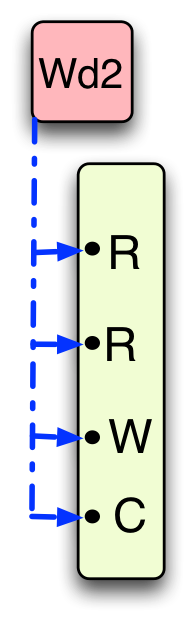
\includegraphics[scale=0.45]{Figures/hb-eg-1}
}
\subcaptionbox {
  \label{fig:hb-eg-2}
} [
  0.25\columnwidth
] {
  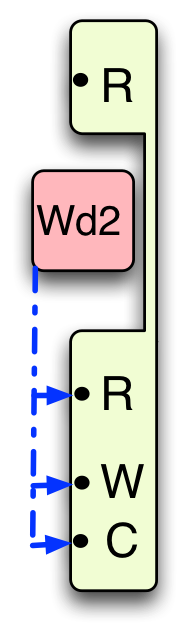
\includegraphics[scale=0.45]{Figures/hb-eg-2}
}
\subcaptionbox {
  \label{fig:hb-eg-3}
} [
  0.25\columnwidth
] {
  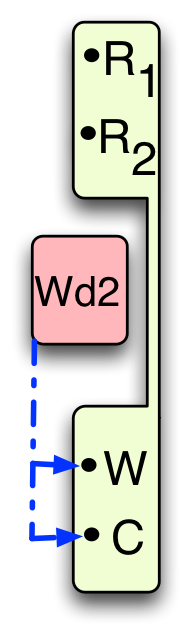
\includegraphics[scale=0.45]{Figures/hb-eg-3}
}
\subcaptionbox {
  \label{fig:hb-eg-4}
}{
  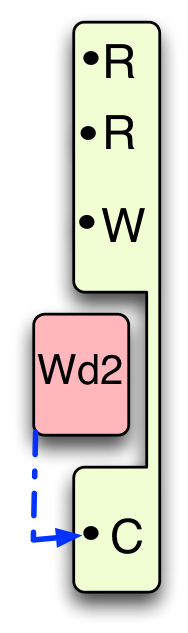
\includegraphics[scale=0.45]{Figures/hb-eg-4}
}


\caption{\small Possible executions for the example in
Fig.~\ref{fig:motiv-eg-1}. Letters R, W and C stand for read, write
and commit, respectively. Each blue dashed arrow represents a $\hbZ$
relationship between all operations of \C{Wd2} and an operation in
\C{Wd1}. $\psi_{SI}$ specification allows $\hbZ$ arrows (hence the
execution) in Fig.~\ref{fig:hb-eg-1}. $\psi_{RC}$ specification allows
$\hbZ$ arrows in
Figs.~\ref{fig:hb-eg-1},~\ref{fig:hb-eg-2},~\ref{fig:hb-eg-3}, and
~\ref{fig:hb-eg-4}.  }
\label{fig:motiv-eg-1-hb}
\vspace*{-8pt}
\end{figure}

For the rely-guarantee approach to be useful, it has to thus constrain
allowed interference in accordance with the chosen level of isolation
associated with a transaction. The first observation we make is that
we can constrain interference by constraining the nature of the
\emph{happens-before} ($\hbZ$) relation, which ultimately dictates
what other transactions become visible to a transaction, or its
constituents, and when. To do so, we axiomatize the $\hbZ$ relation to
capture the interference characteristics of different isolation levels
as their specifications. Two such specifications are
shown\footnote{Note that specifications presented here are solely for
illustration. The actual specifications described in
\S\ref{sec:ansi-isolation} are more nuanced.} in
Fig.~\ref{fig:interference-ex}. The \iso{Read Committed} specification
($\psi_{RC}$) allows an operation $\eta_1$ of a transaction $T_1$ to
happen-before an operation $\eta_2$ of another transaction $T_2$ only
if every operation in $T_1$ (including its commit) happens-before
$\eta_2$ (we let $T_1 \hboar \eta_2$ denote this). The specification
does not require $T_1$ to execute and commit before all operations of
$T_2$, thus allowing it to interfere in $T_2$, just as \C{Wd2}
interferes in \C{Wd1} in Fig.~\ref{fig:motiv-eg-1-a}. The
\iso{Snapshot Isolation} specification ($\psi_{SI}$) requires two
transactions that write to the same variable (denoted $\wrstoar$) to be
related by happens-before.  This effectively prohibits interference
due to actions in $T_1$ being interleaved in $T_2$ (or, vice versa). 

Fig.~\ref{fig:motiv-eg-1-hb} is a visualization of $\hbZ$ from \C{Wd2}
to \C{Wd1} allowed by $\psi_{RC}$ and $\psi_{SI}$. Arrows in all
executions are legal under $\psi_{RC}$ because in no execution does an
operation from \C{Wd2} happen-before an operation of \C{Wd1} without
the commit of \C{Wd2} also happening before the operation of \C{Wd1}.
$\psi_{SI}$ however disallows $\hbZ$ arrows (hence executions) in
Figs.~\ref{fig:hb-eg-2},~\ref{fig:hb-eg-3}, and~\ref{fig:hb-eg-4}
because such arrows establish $\hbZ$ edges between (operations in)
\C{Wd2} and only a subset of the operations in \C{Wd1}. Since the
result of an operation (\eg a read) depends on what happens before
that operation, the structure of the $\hbZ$ relation ultimately
dictates the final result of the program. The arrows in
Figs.~\ref{fig:hb-eg-1} and~\ref{fig:hb-eg-2} denote $\hbZ$
relationships that do not affect the value of \C{B} in a way that
causes the program to violate its post-condition. In contrast, arrows
in Figs.~\ref{fig:hb-eg-3} and~\ref{fig:hb-eg-4} denote $\hbZ$
relationships that lead to the violation of the post-condition. The
task of the reasoning framework is to determine if \emph{all} $\hbZ$
relationships allowed by an isolation level lead to the satisfaction
of the post-condition.

% There is a $\hb$ edge (first dashed) that is allowed by RC but
% prohibited by SI, which nonetheless does not lead to invariant
% violation. 

The specification of an isolation level encodes its interference
characteristics as constraints over the $\hbZ$ relation. However, for
this to be useful in reasoning about programs, the rely-guarantee
framework should be able to use the specification to determine if an
interference is valid or not, allowing the programmer to only focus on
valid interferences. Our second observation is that this is possible
if the reasoning framework adequately tracks $\hbZ$ at each program
point, while preserving $\hbZ$ constraints as invariants between
program points. An interference that leads to the violation of $\hbZ$
constraints (i.e., an invalid interference) is thus automatically
prohibited. For instance, consider the program point after the write
to \C{B} in \C{Wd1}. The expected invariant ($\phi$) at that program
point is shown below ($\committed$ stands for ``committed''):

\begin{smathpar}
\begin{array}{c}
 \neg\committed(\C{Wd1}) \conj \C{Wd1} \wrstoar \C{B}  \conj 
    (\neg\committed(\C{Wd2}) \Rightarrow \C{B = k-a1}) \\
    \conj (\committed(\C{Wd2})
                \Rightarrow \C{B = k-a1-a2})
\end{array}
\end{smathpar}

\noindent $\phi$ asserts that \C{Wd1} is not yet committed, and that
it wrote to \C{B}, and the value of \C{B} is either \C{k-a1-a2} or
\C{k-a1} depending on whether or not \C{Wd2} is committed. If $\phi$
remains invariant until \C{Wd1} commits, then the post-condition (\C{B
= k-a1-a2}) can be established easily. However, an interference from
\C{Wd2} at this stage (captured by the last dashed arrow in
Fig.~\ref{fig:motiv-eg-1-hb}) may violate the invariant by writing
$\C{k-a2}$ to \C{B} and committing \C{Wd2}, thus leading to
$\committed(\C{Wd2}) \Rightarrow \C{B=k-a2}$. Fortunately,
\iso{Snapshot Isolation} prevents this interference, and this can be
shown by demonstrating that an interference from \C{Wd2} starting from
an execution state that satisfies $\psi_{SI} \wedge \phi$ leads to an
execution state where neither $\C{Wd2} \hboar \C{Wd1}$ nor $\C{Wd1}
\hboar \C{Wd2}$ holds; $\C{Wd2} \hboar \C{Wd1}$ does not hold because
\C{Wd1}'s write to \C{B} clearly happened before \C{Wd2}'s commit, and
$\C{Wd1} \hboar \C{Wd2}$ does not hold because \C{Wd1} has not yet
committed, while \C{Wd2} has already begun. Since \C{Wd2} also writes
to \C{B}, this violates the $\psi_{SI}$ constraint which we assume to
be an invariant. A proof that the post-condition holds now follows
from the contradiction. It is informative to note that if the
invariant is $\psi_{RC}$ instead of $\psi_{SI}$, we cannot derive a
contradiction and we cannot rule out the interference, which
(rightfully) causes  the proof to fail.

Implicit in the above discussion is the assumption of a strongly
consistent ({\sc sc}) store that guarantees the visibility of all
previously committed transactions. An {\sc sc} semantics can be built
into the reasoning framework, leading to a proof system tailor-made
for such stores.  However, for the reasoning framework to be truly
useful, it should be capable of handling different consistency
semantics, supporting stores that are weaker than {\sc sc} (e.g.,
causally or eventually consistent), and should be able to reconcile
conflicts between consistency and isolation constraints.  We
demonstrate how our reasoning framework makes this possible in the
following sections.

%% We have thus far assumed a strongly consistent ({\sc sc}) store that,
%% in the absence of transactions with special isolation requirements,
%% makes the effects of any operation immediately visible to all
%% subsequent operations. The natural behaviour of {\sc sc} to totally
%% order all operations w.r.t. the $\hbZ$ relation could be in conflict
%% with the constraints imposed by weak isolation. To meet the
%% requirements of weaker isolation levels, say {\sc rc}, the store has
%% to adapt itself to \emph{hide} the effects of concurrent transactions
%% until they are committed. Once committed though, effects need to be
%% immediately visible to subsequent operations. This semantics can be
%% built into the reasoning framework, leading to a proof system
%% tailor-made for such stores. However, for the reasoning framework to
%% be truly useful, it has to be parametric over different consistency
%% semantics, supporting stores that are weaker than {\sc sc} (e.g.,
%% causally or eventually consistent), and should be able to reconcile
%% conflicts between consistency and isolation constraints.  We
%% demonstrate how our reasoning framework makes this possible in the
%% following sections.
